%\documentclass[14pt]{beamer}
\documentclass{beamer}

\usetheme{Copenhagen}
% \usetheme{Boadilla}
% \usecolortheme{beaver}
\setbeamercolor{alerted text}{fg=orange}
\setbeamercolor{background canvas}{bg=white}
\setbeamercolor{block body alerted}{bg=normal text.bg!90!black}
\setbeamercolor{block body}{bg=normal text.bg!90!black}
\setbeamercolor{block body example}{bg=normal text.bg!90!black}
\setbeamercolor{block title alerted}{use={normal text,alerted text},fg=alerted text.fg!75!normal text.fg,bg=normal text.bg!75!black}
\setbeamercolor{block title}{bg=blue}
\setbeamercolor{block title example}{use={normal text,example text},fg=example text.fg!75!normal text.fg,bg=normal text.bg!75!black}
\setbeamercolor{fine separation line}{}
\setbeamercolor{frametitle}{fg=white}
\setbeamercolor{item projected}{fg=white}
\setbeamercolor{normal text}{bg=white,fg=black}
\setbeamercolor{palette sidebar primary}{use=normal text,fg=normal text.fg}
\setbeamercolor{palette sidebar quaternary}{use=structure,fg=structure.fg}
\setbeamercolor{palette sidebar secondary}{use=structure,fg=structure.fg}
\setbeamercolor{palette sidebar tertiary}{use=normal text,fg=normal text.fg}
\setbeamercolor{section in sidebar}{fg=brown}
\setbeamercolor{section in sidebar shaded}{fg=grey}
\setbeamercolor{separation line}{}
\setbeamercolor{sidebar}{bg=red}
\setbeamercolor{sidebar}{parent=palette primary}
\setbeamercolor{structure}{bg=black, fg=white!30!blue!60!green}
\setbeamercolor{subsection in sidebar}{fg=brown}
\setbeamercolor{subsection in sidebar shaded}{fg=grey}
\setbeamercolor{title}{fg=white}
\setbeamercolor{titlelike}{fg=white}

\frenchspacing

% Language packages
\usepackage[utf8]{inputenc}
\usepackage[T1]{fontenc}
\usepackage[magyar]{babel}

% AMS
\usepackage{amssymb,amsmath}

% Graphic packages
\usepackage{graphicx}

% Syntax highlighting
\usepackage{listings}

\usepackage{tikz}

\title[Használati módokra optimalizált ütemezési stratégiák]{Használati módokra optimalizált \\ ütemezési stratégiák}
\author[Vass Dávid Attila]{\textbf{Vass Dávid Attila}}
\institute[]{Miskolci Egyetem, Alkalmazott Matematikai Intézeti Tanszék}
\date{2021. június 16.}

\begin{document}
\begin{frame}
\maketitle
\end{frame}

\begin{frame}
\frametitle{Bevezetés}
\begin{itemize}

\item A mai világban nehezen elképzelhetőnek tűnnek azok a számítógépek, amik egyszerre csak egyetlen folyamatot képesek futtatni.
%A definiciója a single-tasking rendszereknek, kicsit értelmét vesztette a modern hardware-eken. 
\item Egy multi tasking rendszer már alapvető követelménynek tekinthető manapság az általános célú operációs rendszerek között. 
%Egy ilyen rendszerben, több proccess verseng egymással és mindenki a processzort szeretné megkapni. Könnyen előfordulhat, hogy száz, akár kétszáz processz is várakozik, de nekünk nincs kétszáz processzorunk, hogy mindenki futni tudjon. Ezt egy "pszeudo párhuzamossággal" éri el a rendszer, ami azt jelenti, hogy váltogatva futnak és ez a váltogatás nagyon gyorsan történik. Egy másodperc alatt akár ezerszer is bekövetkezhet.
\item A kernel egyik fő feladata a CPU kiosztása, egy processz számára. El kell döntenie, hogy melyik futásra kész állapotú processz kapja meg a CPU-t.
\item Processz ütemezőnek hívják, a kernelnek azt a részét, ami ennek az eldöntésével foglalkozik.
\item Az elkészített alkalmazás célja, hogy a segítségével az adott felhasználási módhoz lehessen igazítani az ütemezési stratégiát. (Hasonlóan, mint a \texttt{tuna} és \texttt{tuned} esetében.)
\end{itemize}
\end{frame}

\begin{frame}
\frametitle{Ütemező optimalizálási stratégiák}
%TODO : O(1), O(n) és CFS ütemező (említés szintjén)
A dolgozat elejében néhány elterjedt ütemezési stratégiát is bemutatok, mint például az $\mathcal{O}(n)$, $\mathcal{O}(1)$ és a Completely Fair Scheduler-t.
A jelenlegi Linux kernel ütemező, a Completely Fair Scheduler és ennek az optimalizálásra kerestem megoldásokat.
% A lineáris idejű $\mathcal{O}(n)$
% Konstans idejű ütemezés $\mathcal{O}(1)
Annak érdekében, hogy ezt megvalósítsam, módosításokat kell végezzek az ütemezőn, amit megtehetek többféleképpen például:
\begin{itemize}

\item Módosítom konkrétan a forráskódot.
%Ezzel a probléma hogy minden módosítás után, újra kell fordítanom a kernelt és ezután kell megfigyelem a módosítások hatásait. Ez elég időigényes és mellesleg a forráskód sem túl rövid. Jelenleg olyan 11ezer sor, a cfs rész

\item Az ütemezőhöz kapcsolódó kernel változókat módosítom.
%Én ezt az utóbbit választottam, mivel ezeknek van egy olyan tulajdonságuk, hogy futásidőben is módosíthatók.
\end{itemize}
\end{frame}

%TODO : Piros-fekete fáról az ábra (ami a dolgozatban is szerepel.)
\begin{frame}
\frametitle{Processz megválasztása a CFS ütemezőben}
\begin{center}
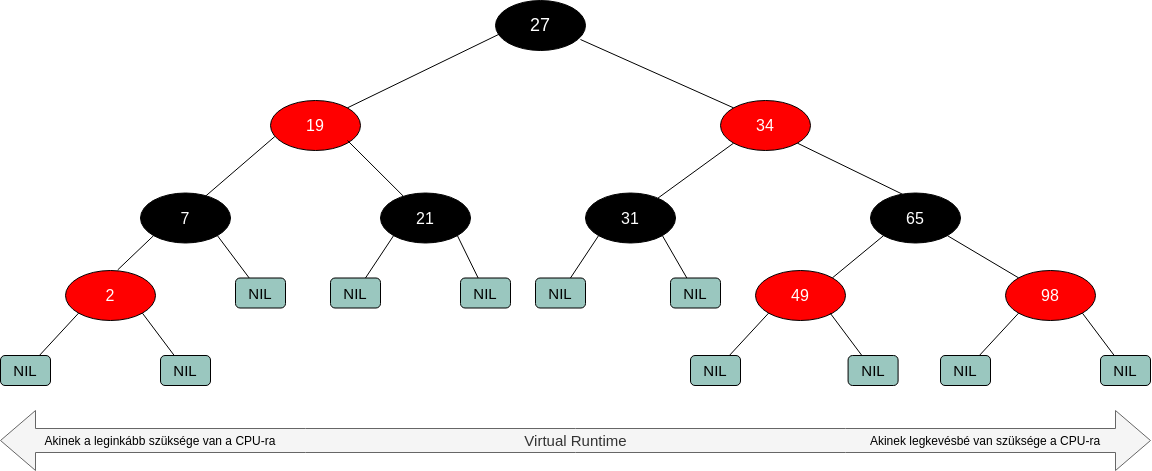
\includegraphics[scale=0.25]{./images/redBlackTree.png}
\end{center}
%A CFS egy piros-fekete fát használ, a listában lévő futtatható taskok kezelésére, hogy egyszerűen megtalálhassa a legkisebb vruntime-mal rendelkező taskot.
%Ez egy saját magát kiegyensúlyozó bináris fa, a bal oldalában a legfontosabb taszkok helyezkednek el.
%A jobb oldalában pedig a kevésbé fontosak.
\end{frame}


\begin{frame}
\frametitle{ Ütemezőhöz kapcsolódó kernel változók}
Az ütemezőhöz és még sok más kernel komponenshez tartozó változót, megtalálhatunk a \texttt{/proc/sys/kernel/} jegyzékben.
\begin{itemize}
\item Fontos, hogy ezek a változók futásidőben is módosíthatók.
\item Minden változóhoz tartozik egy intervallum, amin belül tetszőlegesen változtatható az értéke. 
\end{itemize} 

Ezek értékeit beállítjuk többféle módon.
\begin{itemize}
\item Felülírjuk konkrétan a fájlban az értéket.
\item Sysctl interface segítségével.
%Én a sysctl interface-es megoldást választottam, mivel egyszerűbbnek tűnt.
\end{itemize}

\end{frame}

\begin{frame}
\frametitle{Sysctl interface}
A \textit{sysctl} interface segítségével lekérdezhetem, módosíthatom a kernel változók aktuális értékeikeit és figyelmeztet arra is, hogy az adott változó értékét ne állítsam az intervallum végpontjain túllépő értékekre.
A konkrét ütemezőhöz kapcsolódó változók amiket módosítottam, a következők.

\begin{itemize}
\item \texttt{sched\_latency\_ns}
%Ez a paraméter kis processz szám esetén jelentős, mivel ebben az esetben ő lesz a maga a időszelet hossza.
\item \texttt{sched\_min\_granularity\_ns}
%Ő az előzővel ellentétben, nagy processz szám esetén érvényesül. A célja hogy egy alsó határként szolgáljon és minden processznek jusson elég idő a futáshoz. Az időszelet mérete a sched_min_gran * processz szám lesz. 
\item \texttt{sched\_wakeup\_granularity\_ns}
%Ez az a minimális idő amelynek el kell telnie, mielőtt a CFS ütemező fontolóra veszi, hogy egy nagyobb \texttt{vruntime} értékkel rendelkező futtatható állapotú folyamattal leváltja, a jelenleg végrehajtás alatt álló taszkot.
%Ez az opció késlelteti a preempció hatásait és csökkenti a túlütemezést.
\item \texttt{sched\_tunable\_scaling}
%Az ütemező hangoló paramétereket milyen mértékben szabályozhatja a kernel, amihez három féle opció is rendelkezésre áll. Ezt a változót 0-ra állítottam mindig, így az én beállításaimat, nem módsította tovább.
\end{itemize}

Ezek mellett még két változón fogok módosításokat végezni, a processz prioritásán és a \texttt{vm.swappiness} kernel változón.
%A prioritás beleszámolódik a processz vruntime változó értékébe, ami a processz megválasztásnál lesz fontos rész.
%A vm.swappiness pedig a swap memória használatot szabályozza. Az értéke 0 és 100 között mozog, 0 esetén nincs swap használat, 100-as értéknél pedig agresszív swap használatot okoz a rendszerben.
%Ez a két plusz változó a felhasználási módok kialakítása miatt voltak fontosak.
\end{frame}

\begin{frame}
\frametitle{Tesztelési környezet}
Az említett változókat tesztelnek kellett, hogy kiderítsem a változtatásuk milyen hatással van a rendszerre.
Ehhez megpróbáltam különböző benchmark típusokat keresni, amivel különböző felhasználási módokat próbáltam szimulálni.
Erre a célra a Phoronix Test Suite programot választottam, mivel számos teszt program elérhető ezen keresztül.
%Tudjuk telepíteni, futtatni és még ilyen automatizált futtatást is tud, bár az a rész nálam nem volt fontos
% Ezek kiválasztásához figyelembe vett szempontokat említeni.
\begin{itemize}
	\item Ebizzy
	\item PI
	%Ők ketten leginkább a processzort próbálták terhelni. Az utóbbi egy szálon.
	\item Fs-Mark
	%Háttértár terhelés
	\item GlMark2
	%Grafikus kártya terhelés
	\item Ctx-Clock
	%Rendszerterhelés
	\item Stream
	%Memória terhelés
	%Kiválasztásnak a szempontjai: 
	% - A program minél hamarabb készítse el a mérési adatokat.
	% - A működése, mégis azért azt próbálja terhelje amire megválasztottam.
	% - Elérhető konfigurációs beállítások.
\end{itemize}
\end{frame}

\begin{frame}
\frametitle{Parameter-test program}
A változókat intervallumaik szerint négy részre szedtem szét és az összes lehetséges beállítással futtattam öt mintát, minden teszt típussal.
Ennek az automatizálására készítettem a \textit{Parameter-test} programot, ami C programozási nyelv felhasználásval készült. 
A program feladatai:
\begin{itemize}
\item Előkészíteni a Phoronix Test Suite programot batch tesztelési módra.
%Itt főként az xml konfigurációs fájlok írására gondolok, de a program itt kapcsolja ki  a \texttt{sched\_tunable\_scaling} változót is.
\item A kernel változók és prioritás értékeit módosítania kell.
\item Amikor végzett a benchmark egy adott mintaszámmal, a kapott értéket le kell mentenie egy fájlba.
\end{itemize}
\end{frame}

\begin{frame}
\frametitle{Parameter-test program}

\begin{columns}
\begin{column}{0.5\textwidth}
\begin{itemize}
\item A programhoz készítettem egy ncurses-es menüt amivel kiválaszthatjuk a tesztet és futás közben láthatjuk, hogy mennyi teszt van még hátra.
\item Maga a teszt egy JSON fájt készít, amibe beleírja az épp aktuális változó értékekkel elért értékekeket.
\item A kimeneti fájl feldolgozását Python segítségével végeztem. 
\end{itemize}
\end{column}

\begin{column}{0.5\textwidth}
\begin{figure}
\begin{center}
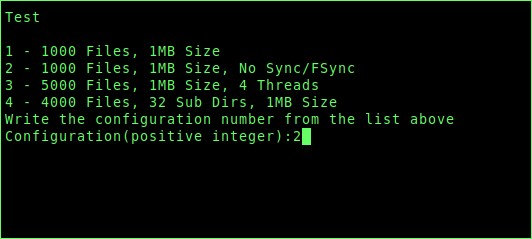
\includegraphics[width=\textwidth]{images/parameter-test-select.png}
\end{center}		
\end{figure}

\begin{figure}
\begin{center}
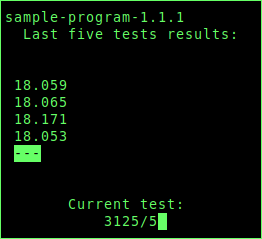
\includegraphics[height=0.3\textheight]{images/parameter-test.png}
\end{center}	
\end{figure}
\end{column}

\end{columns}
\end{frame}


\begin{frame}
\frametitle{SchedulerTuneML}
A \textit{SchedulerTuneML} program Jupyter notebook-ban készült. A gépi tanulás eszközkészletével oldottam meg a paraméterek hangolását.

\medskip

Feladai:
\begin{itemize}
\item A \textit{parameter-test} program által készített JSON fájlokat feldolgozza.
\item A fájlokból kinyert adatokat elemezze.
\item Készítse el az adathalmazt.
\item Miután a gépi tanulás befejeződött, tegyen javaslatokat a kernel változók értékeinek módosítására, az adott felhasználási módhoz viszonyítva.
\end{itemize}   

\end{frame}


\begin{frame}
\frametitle{SchedulerTuneML}

\begin{itemize}
\item A model öt bemenettel, illetve öt kimenettel rendelkezik, és egy rejtett réteget választottam a topológia kialakításához.
%Ez azt jelenti, hogy az adathalmazban az egyes mintáknál, megtalálhatók a jellegek (\textit{features}), illetve az elvárt eredmények is (\textit{labels}).
\item Mivel a kernel változók intervallumait négy részre szedtem szét a teszteléseknél, így egy klasszifikációs algoritmust választottam a model betanítására.
\end{itemize} 

\end{frame}


\begin{frame}
	\frametitle{SchedulerTuneML -- A mesterséges neurális háló felépítése}

\begin{center}
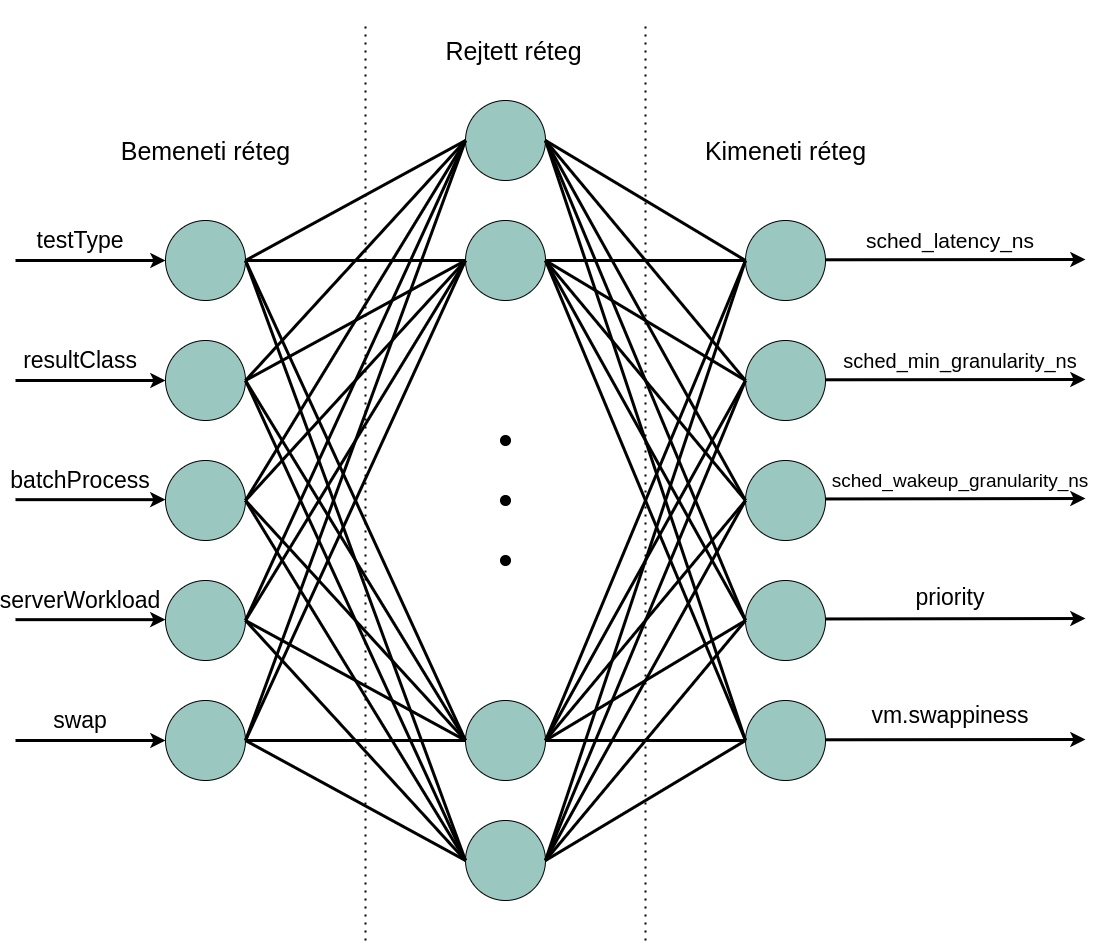
\includegraphics[scale=0.2]{images/neuralNetwork.png}
\end{center}

\end{frame}

\begin{frame}
\frametitle{Teszt eredmények}

Minden teszthez készítettem összesítő ábrákat, külön az elért eredményekhez és a paraméterekhez.
Ezeken megfigyelhető az eredmények eloszlása és hogy mely változók bizonyultak hasznosabbnak a tesztek során.

\begin{figure}
\begin{center}
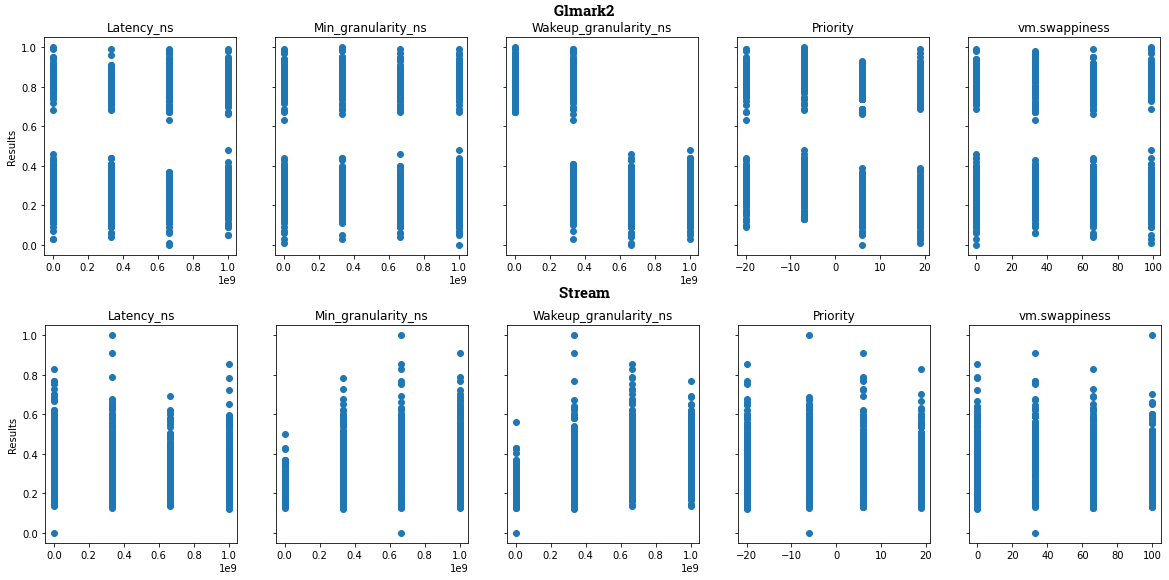
\includegraphics[height=0.5\textheight]{images/graphicsAndMemoryBenchmarkValue.png}
%Ahogy látható, a két benchmark teszteredményeit hasonlónak mondhatjuk. Mindkettőnél megfigyelhető egy "hézag", ami %elválasztja a jobb és a rossz eredményeket. Az eredmények romlása akkor jelentkezik amikor a 
%\texttt{sched\_wakeup\_granularity\_ns} változóhoz nagyobb értékét állítunk, mint a \texttt{sched\_latency\_ns} %fele. Ekkor sajnos a kis időciklusú taszkok nem lesznek képesek versenyezni a többi folyamattal amikor a %processzort éppen nagy terhelés alatt áll.
\end{center}	
\end{figure}

\end{frame}

\begin{frame}
\frametitle{Teszt eredmények}

\begin{figure}
	\begin{center}
		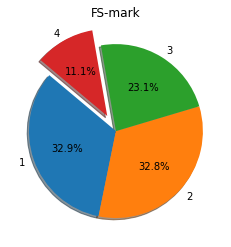
\includegraphics[height=0.62\textheight]{images/diskBenchmarkValue.png}
		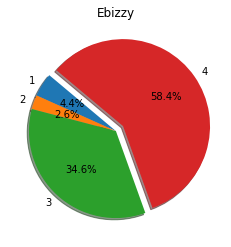
\includegraphics[height=0.62\textheight]{images/cpuBenchmarkValue.png}
	\end{center}	
\end{figure} 

\end{frame}


\begin{frame}
A Red Hat által készített Tuned program, egy rendszer hangoló szolgáltatás amely elérhető GNU/Linux-on.
%A tuned-ben profilok alapján hangolhatjuk a rendszerünket és én összehasonlítottam a készült MachineLearning programot két tuned profillal.
%Ehhez a már bemutatott benchmarkokat használtam fel újra.
\frametitle{Teszt eredmények}
\begin{figure}
	\begin{center}
		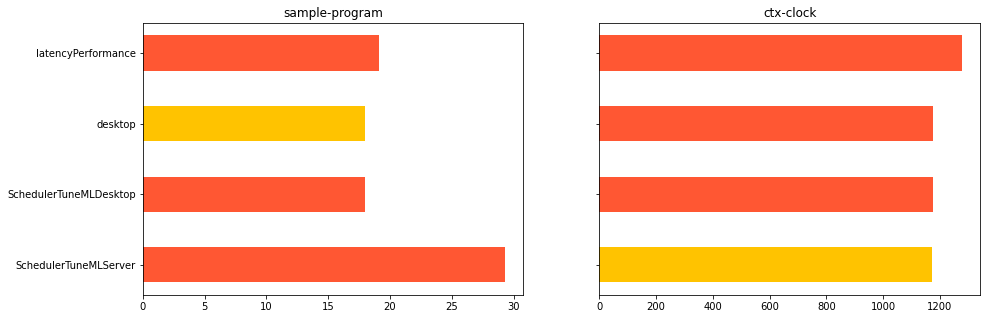
\includegraphics[height=0.4\textheight]{images/tunedAndSchedulerTuneMLCompareSampleprogramCtxclock.png}
	\end{center}	
\end{figure} 
\end{frame}


\begin{frame}
\frametitle{Teszt eredmények}
\begin{figure}
	\begin{center}
		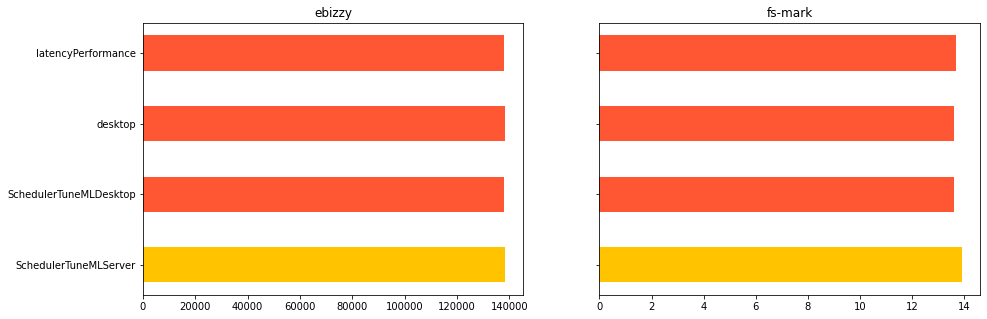
\includegraphics[height=0.4\textheight]{images/tunedAndSchedulerTuneMLCompareEbizzyAndFsMark.png}
	\end{center}	
\end{figure} 
\end{frame}

\begin{frame}
	\frametitle{Összegzés}
	
\begin{itemize}
	\item Áttekintésre került a Linux kernel ütemezője, annak különféle algoritmusai.
	\item A felhasználási módokhoz választottam egy Phoronix benchmark-ot.
	\item Elkészült egy ncurses alapú interfész a benchmark-ok futtatásához.
	\item Mesterséges neurális háló segítségével sikerült becslést adni az adott benchmark-nak megfelelő felhasználási mód optimális paramétereire.
	\item Mérésekkel sikerült alátámasztani az elkészített módszer helyességét.
\end{itemize}
	
\end{frame}

\begin{frame}
	\frametitle{Felhasznált (fontosabb) irodalmak}
	
	\begin{itemize}
		\item Robert Love: Linux Kernel Development, Addison-Wesley, 2010.
		\item Chester Rebeiro: CPU scheduling, 2020.
		\item Red Hat: How to start a process with the deadline scheduler, 2019.
\item Phoronix Media. Phoronix test suite, 2021.
		\item Mohamad H Hassoun et al. Fundamentals of artificial neural networks. MIT press, 1995.
	\end{itemize}
	
\end{frame}

\begin{frame}
\frametitle{\ }
\begin{center}
\Huge \textbf{Köszönöm a figyelmet!}
\end{center}
\end{frame}


\end{document}

